\documentclass{patmorin}
\listfiles
\usepackage[utf8]{inputenc}
\usepackage{amsthm,amsmath,graphicx}
\usepackage{pat}
\usepackage[letterpaper]{hyperref}
\usepackage[dvipsnames]{color}
\definecolor{linkblue}{named}{Blue}
\hypersetup{colorlinks=true, linkcolor=linkblue,  anchorcolor=linkblue,
citecolor=linkblue, filecolor=linkblue, menucolor=linkblue, pagecolor=linkblue,
urlcolor=linkblue, pdfcreator=Me, pdfproducer=Me} \setlength{\parskip}{1ex}

\usepackage{array}


% To reduce space in lists
\usepackage{enumitem}  
\setlist{noitemsep}

%\usepackage[skip=0pt]{caption}

\title{\MakeUppercase{More Turán-Type Theorems for Triangles in Convex Point Sets}\thanks{This research is partially funded by NSERC.}}
\author{Authors TBD}


\newcommand{\edgea}{\raisebox{-.1ex}{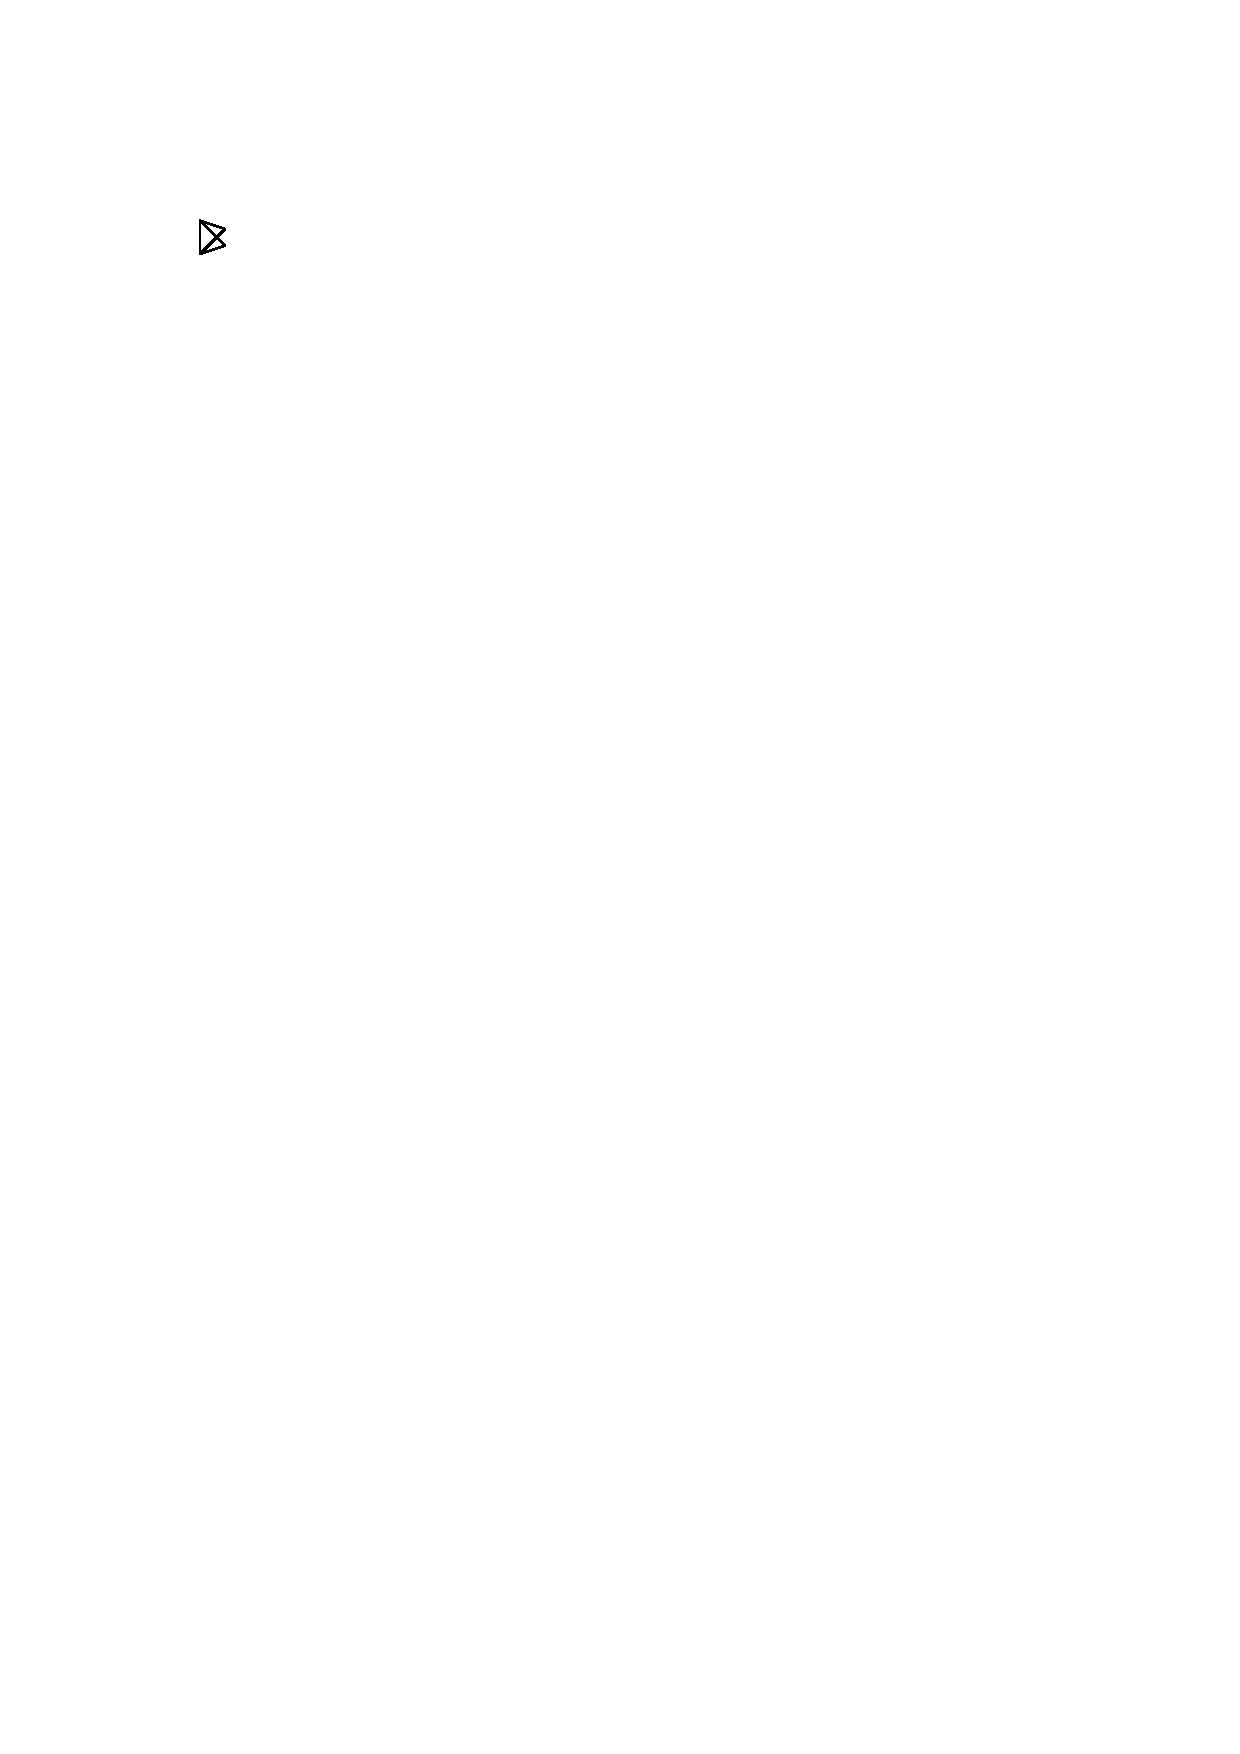
\includegraphics[height=1.6ex]{figs/triangles-edge-1}}}
\newcommand{\edgeb}{\raisebox{-.1ex}{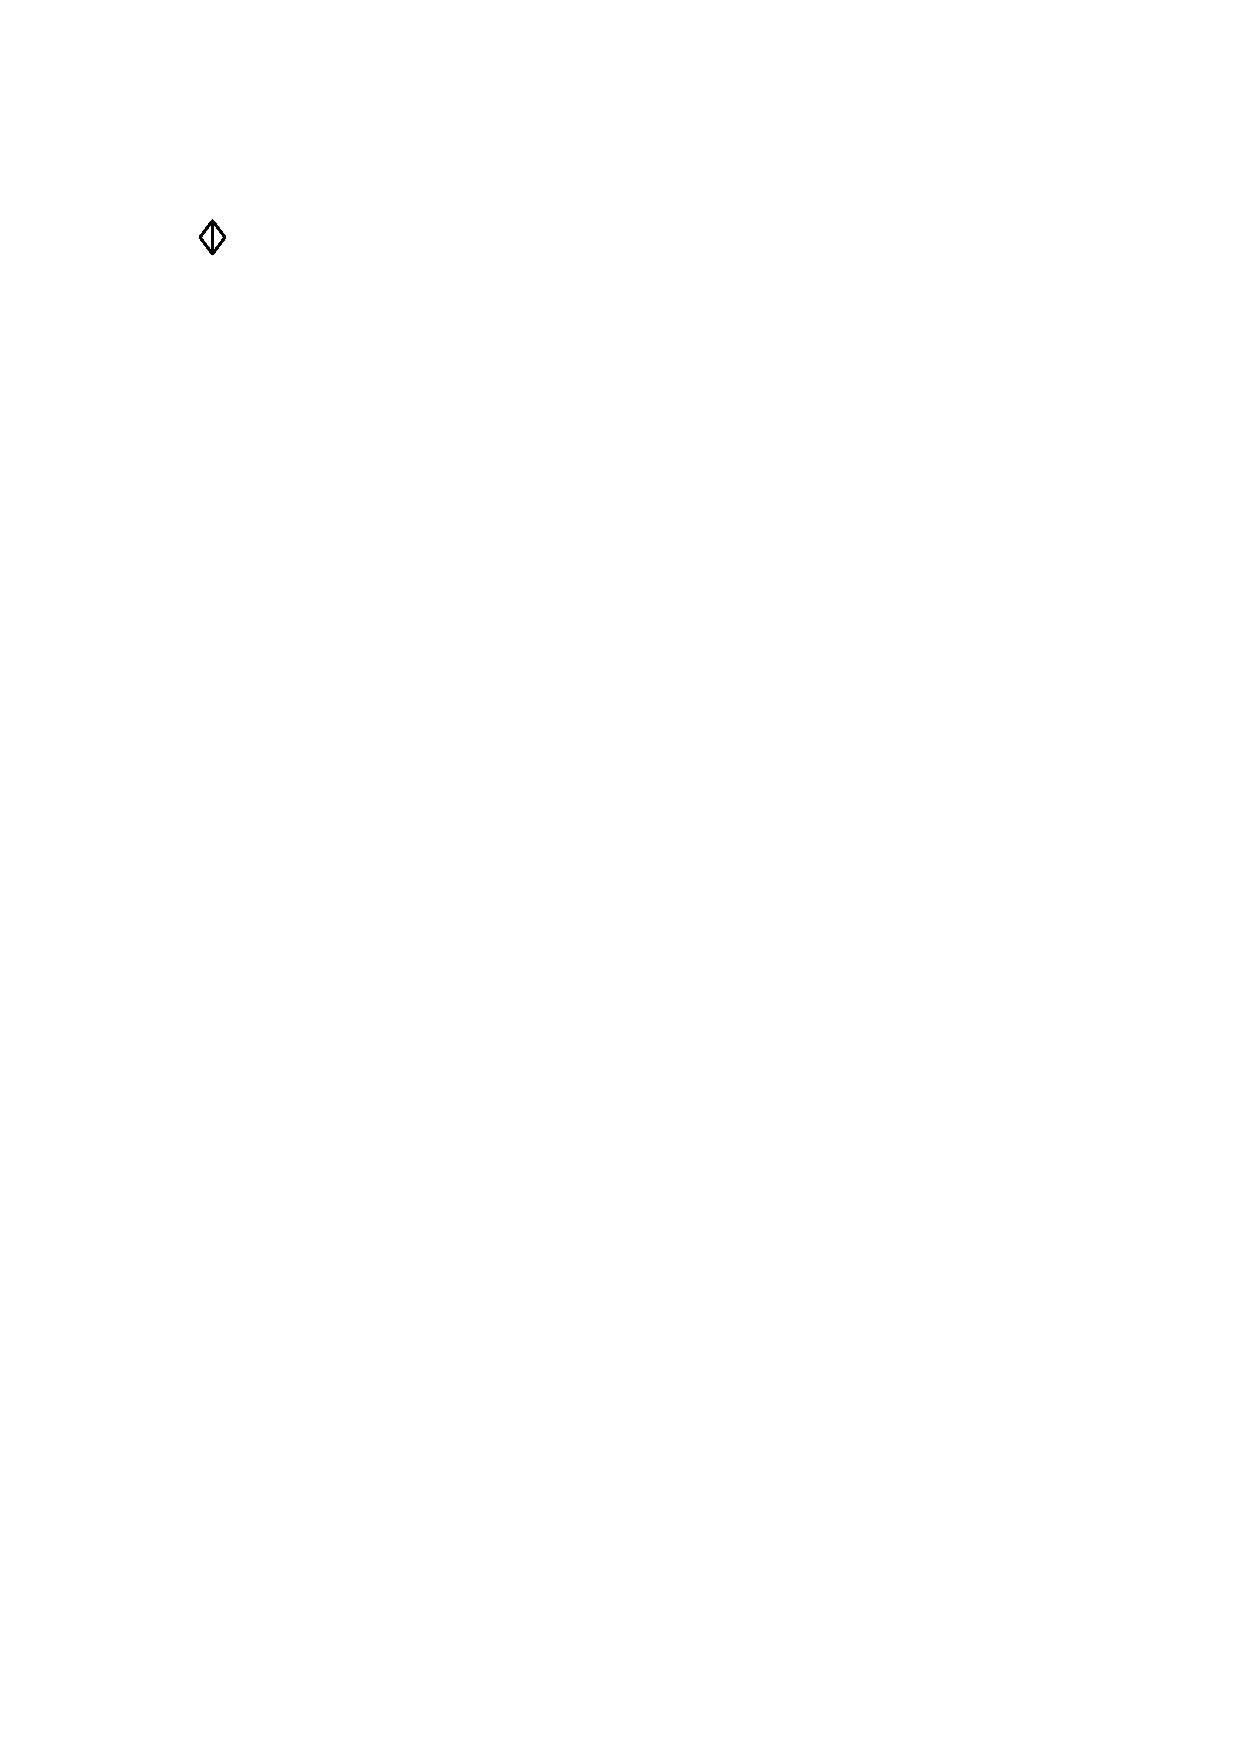
\includegraphics[height=1.6ex]{figs/triangles-edge-2}}}


\newcommand{\vertexa}{\raisebox{-.1ex}{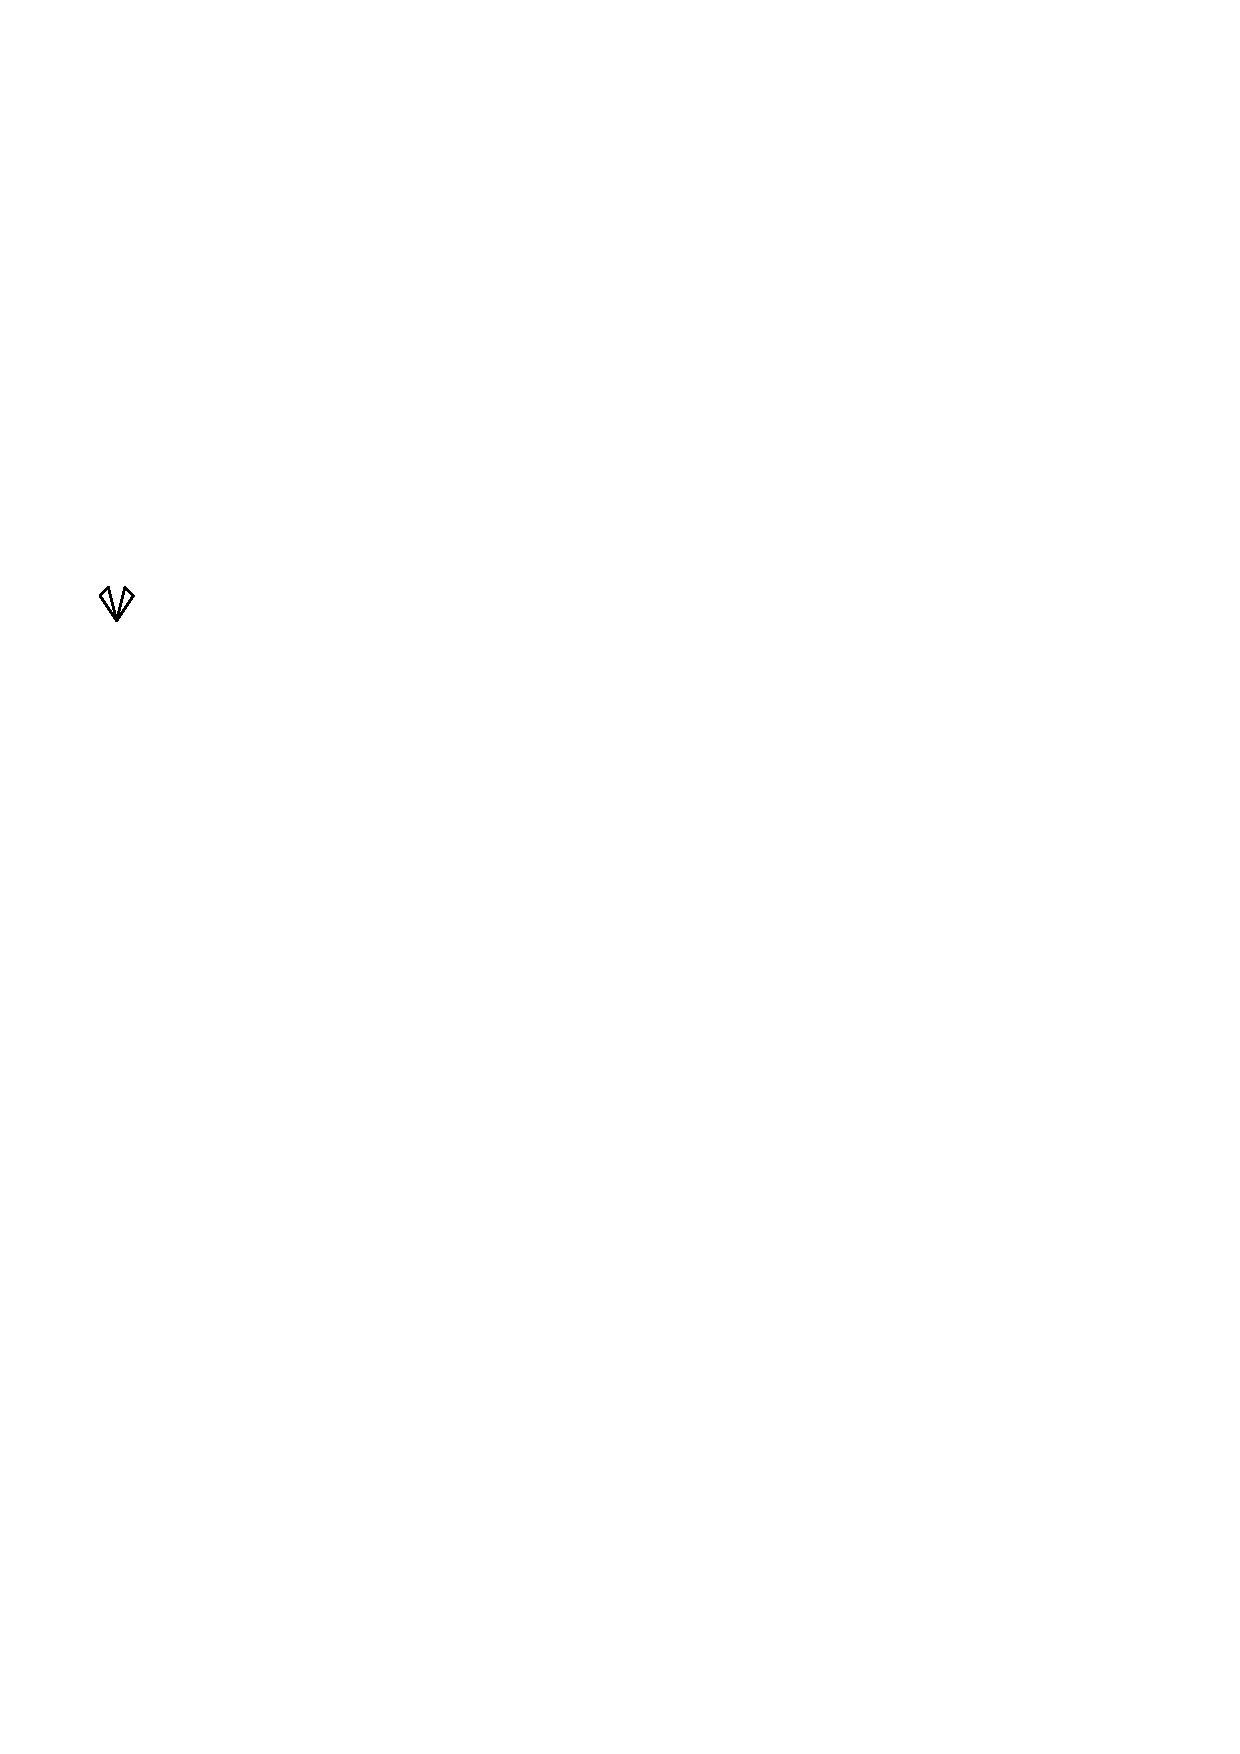
\includegraphics[height=1.6ex]{figs/triangles-vertex-1}}}
\newcommand{\vertexb}{\raisebox{-.1ex}{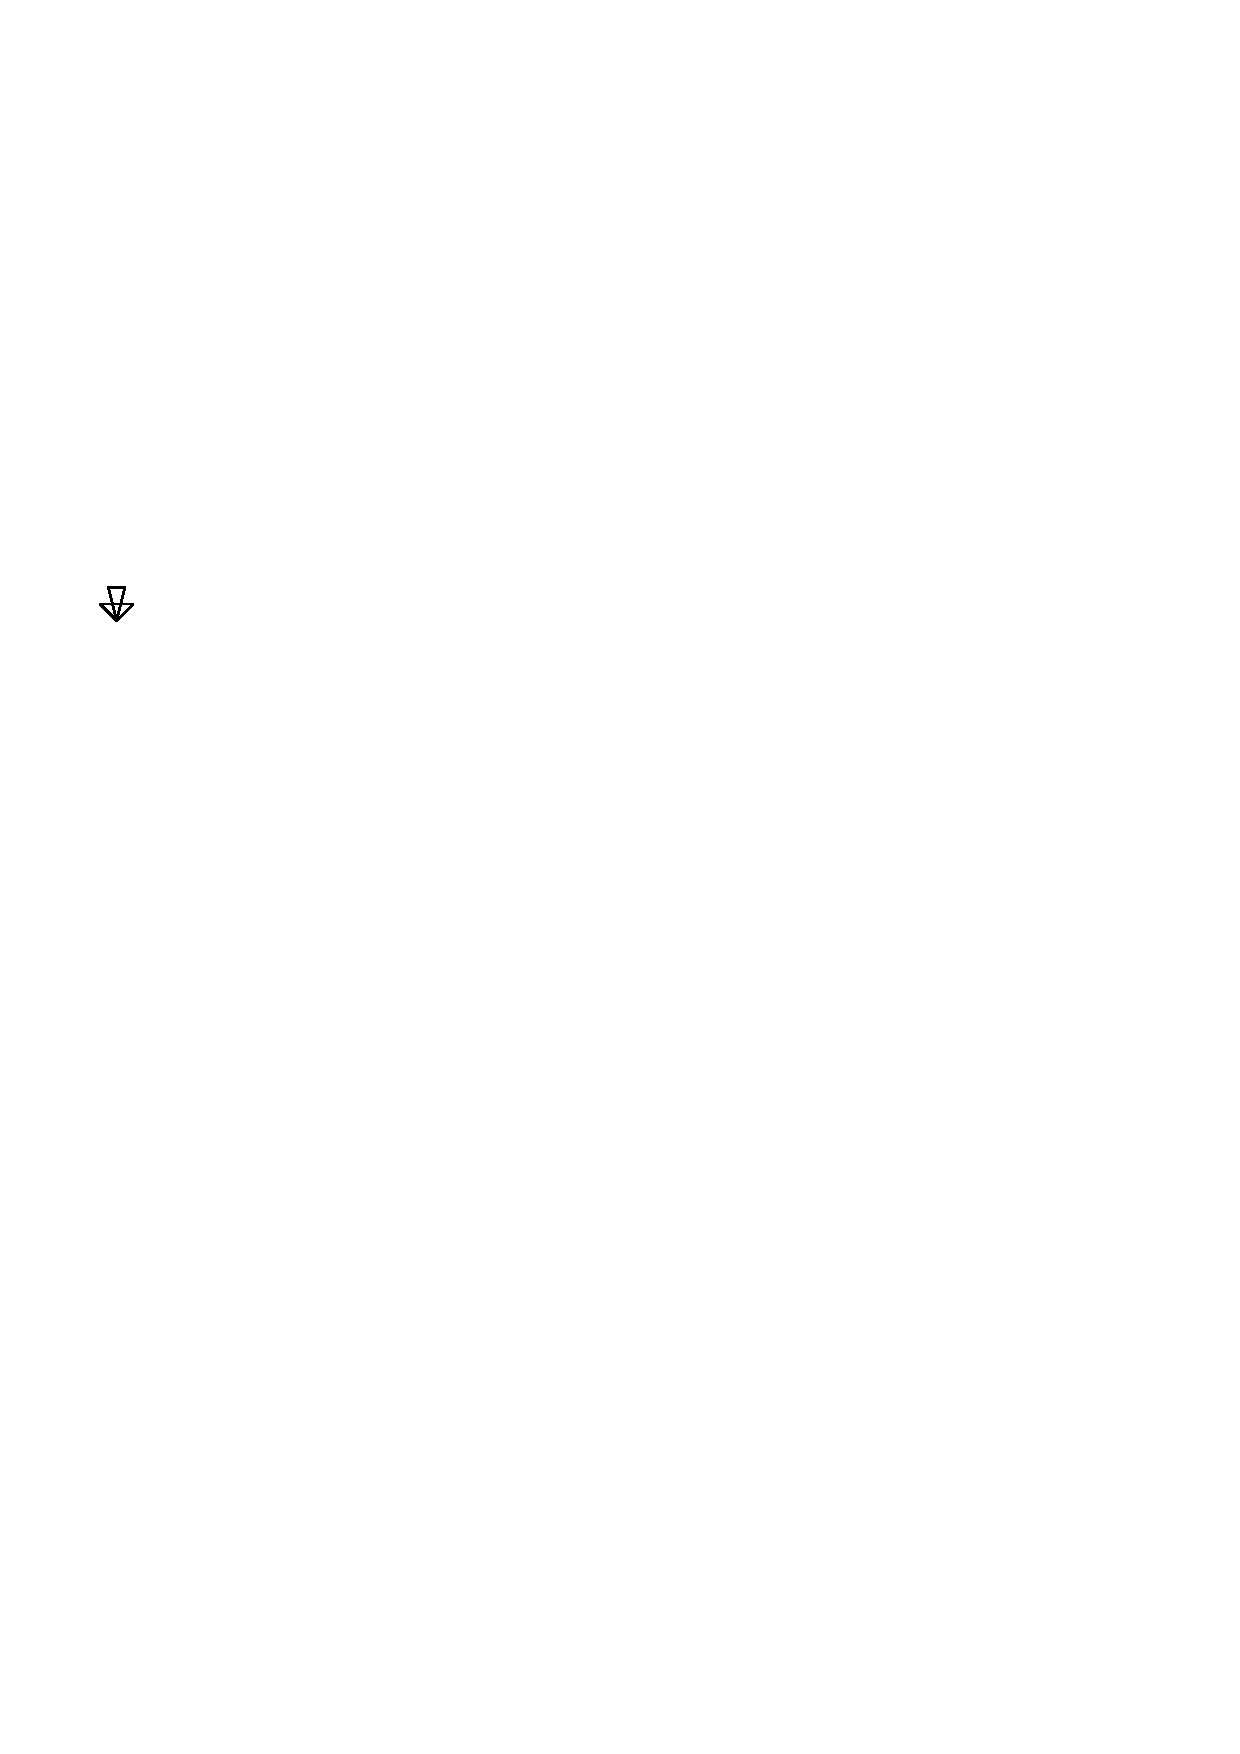
\includegraphics[height=1.6ex]{figs/triangles-vertex-2}}}
\newcommand{\vertexc}{\raisebox{-.1ex}{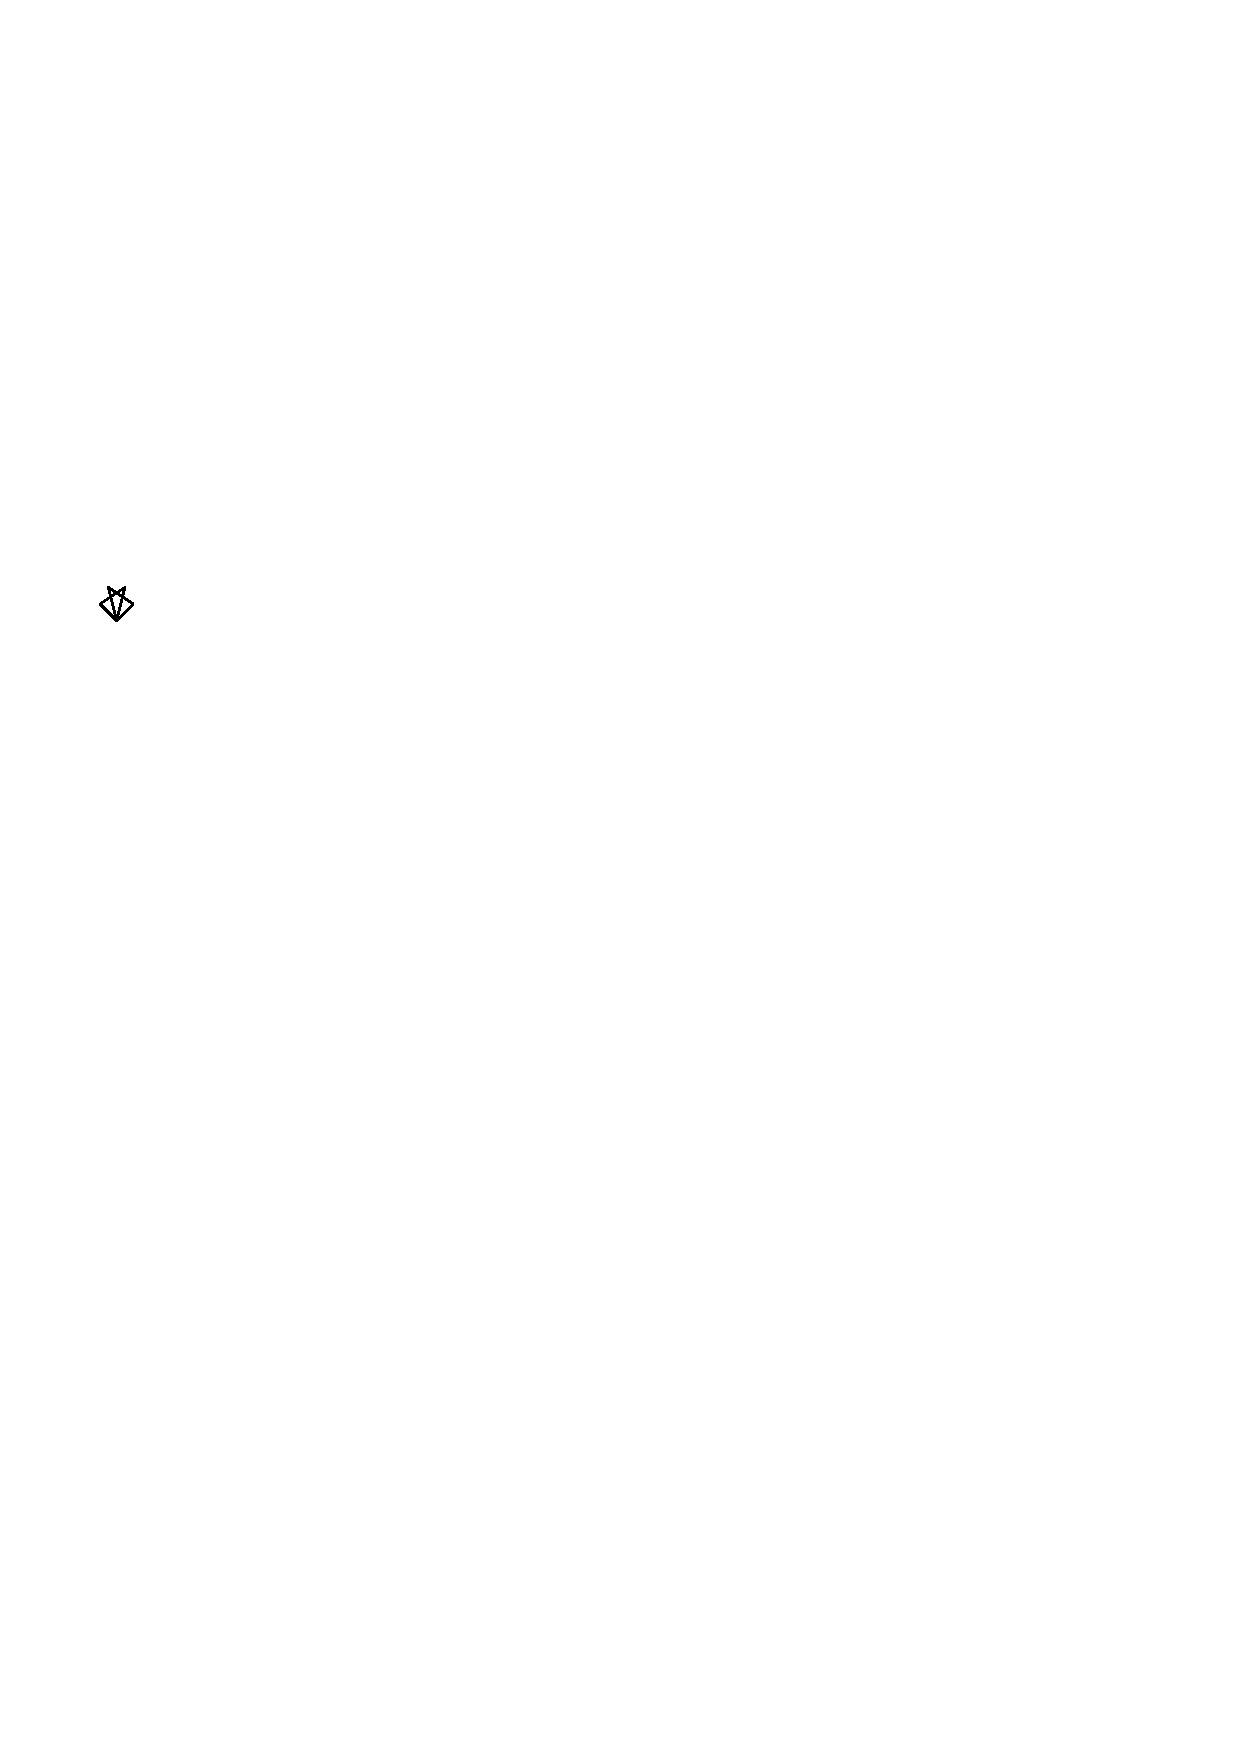
\includegraphics[height=1.6ex]{figs/triangles-vertex-3}}}

\newcommand{\disjointa}{\raisebox{-.1ex}{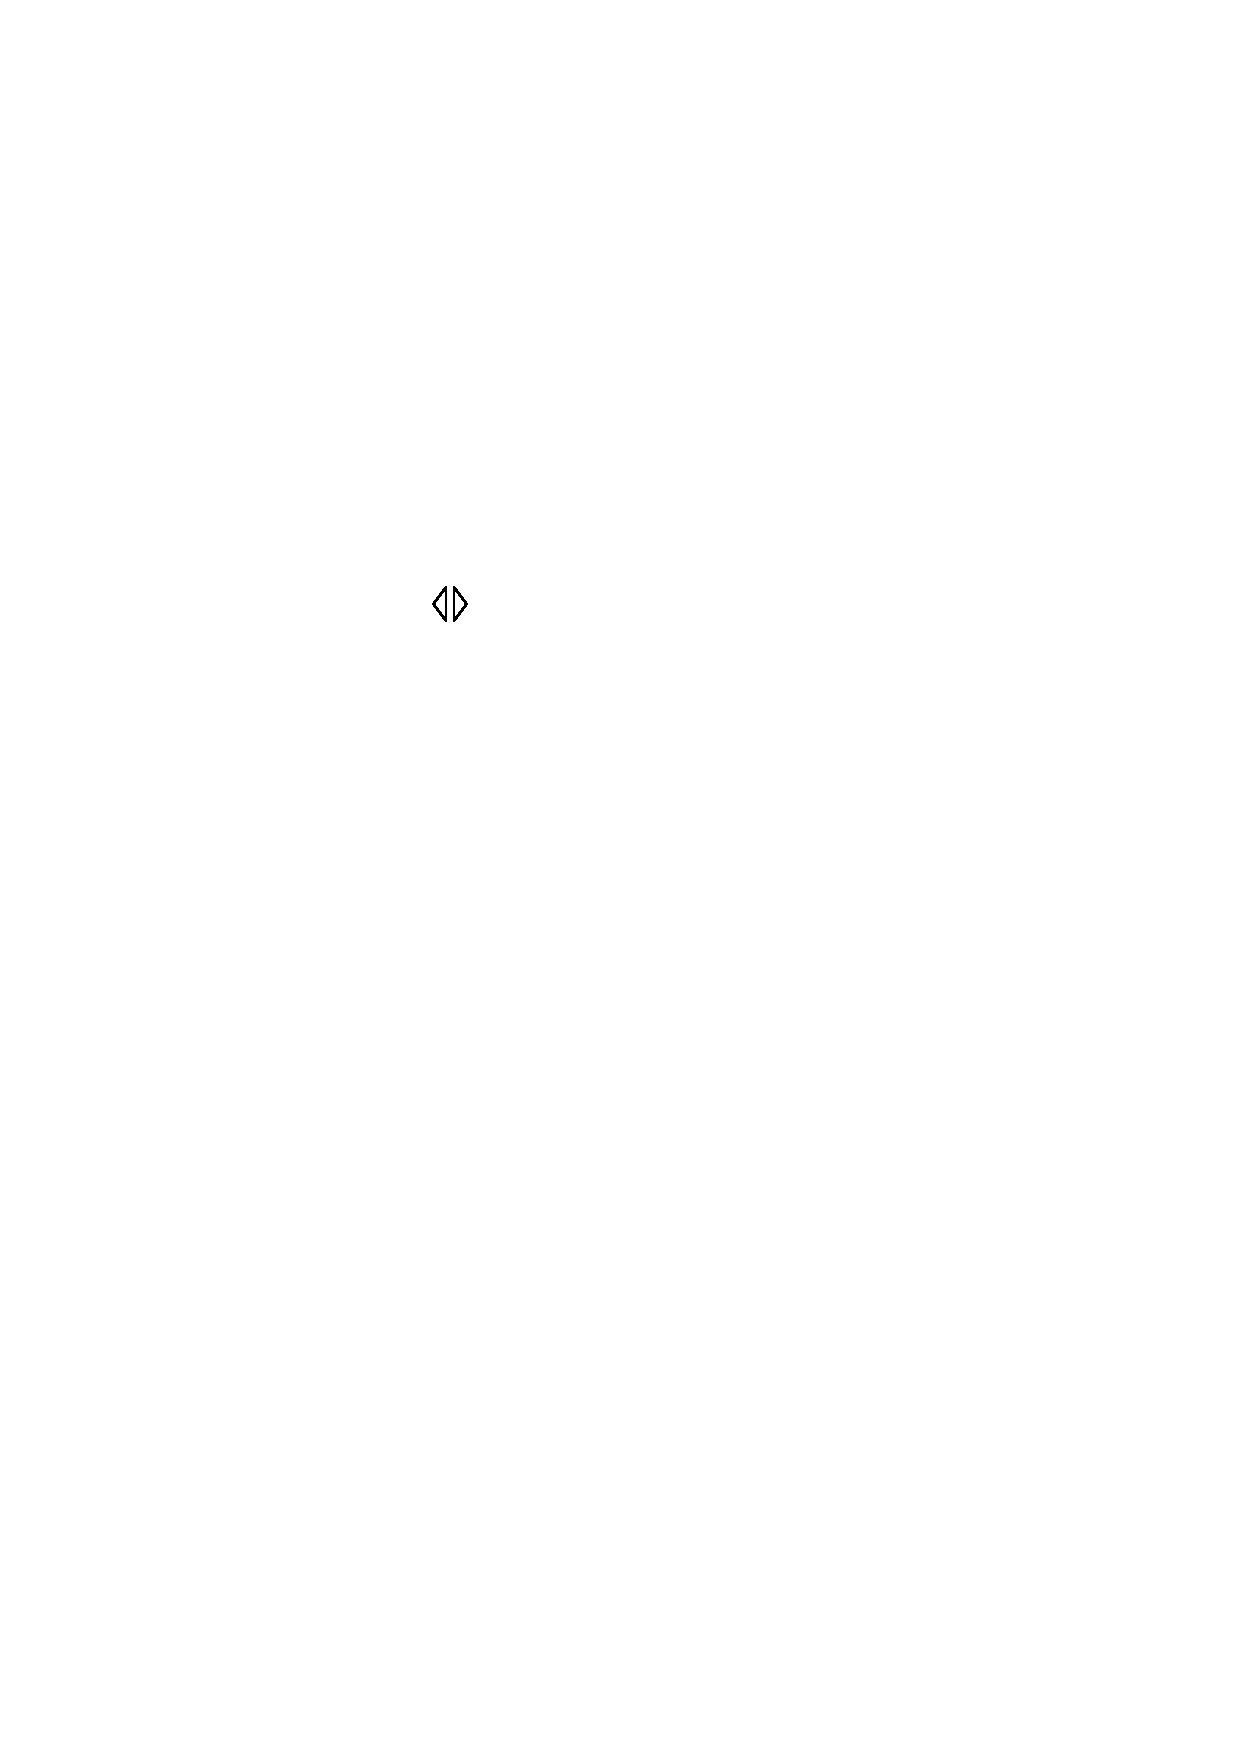
\includegraphics[height=1.6ex]{figs/triangles-disjoint-1}}}
\newcommand{\disjointb}{\raisebox{-.1ex}{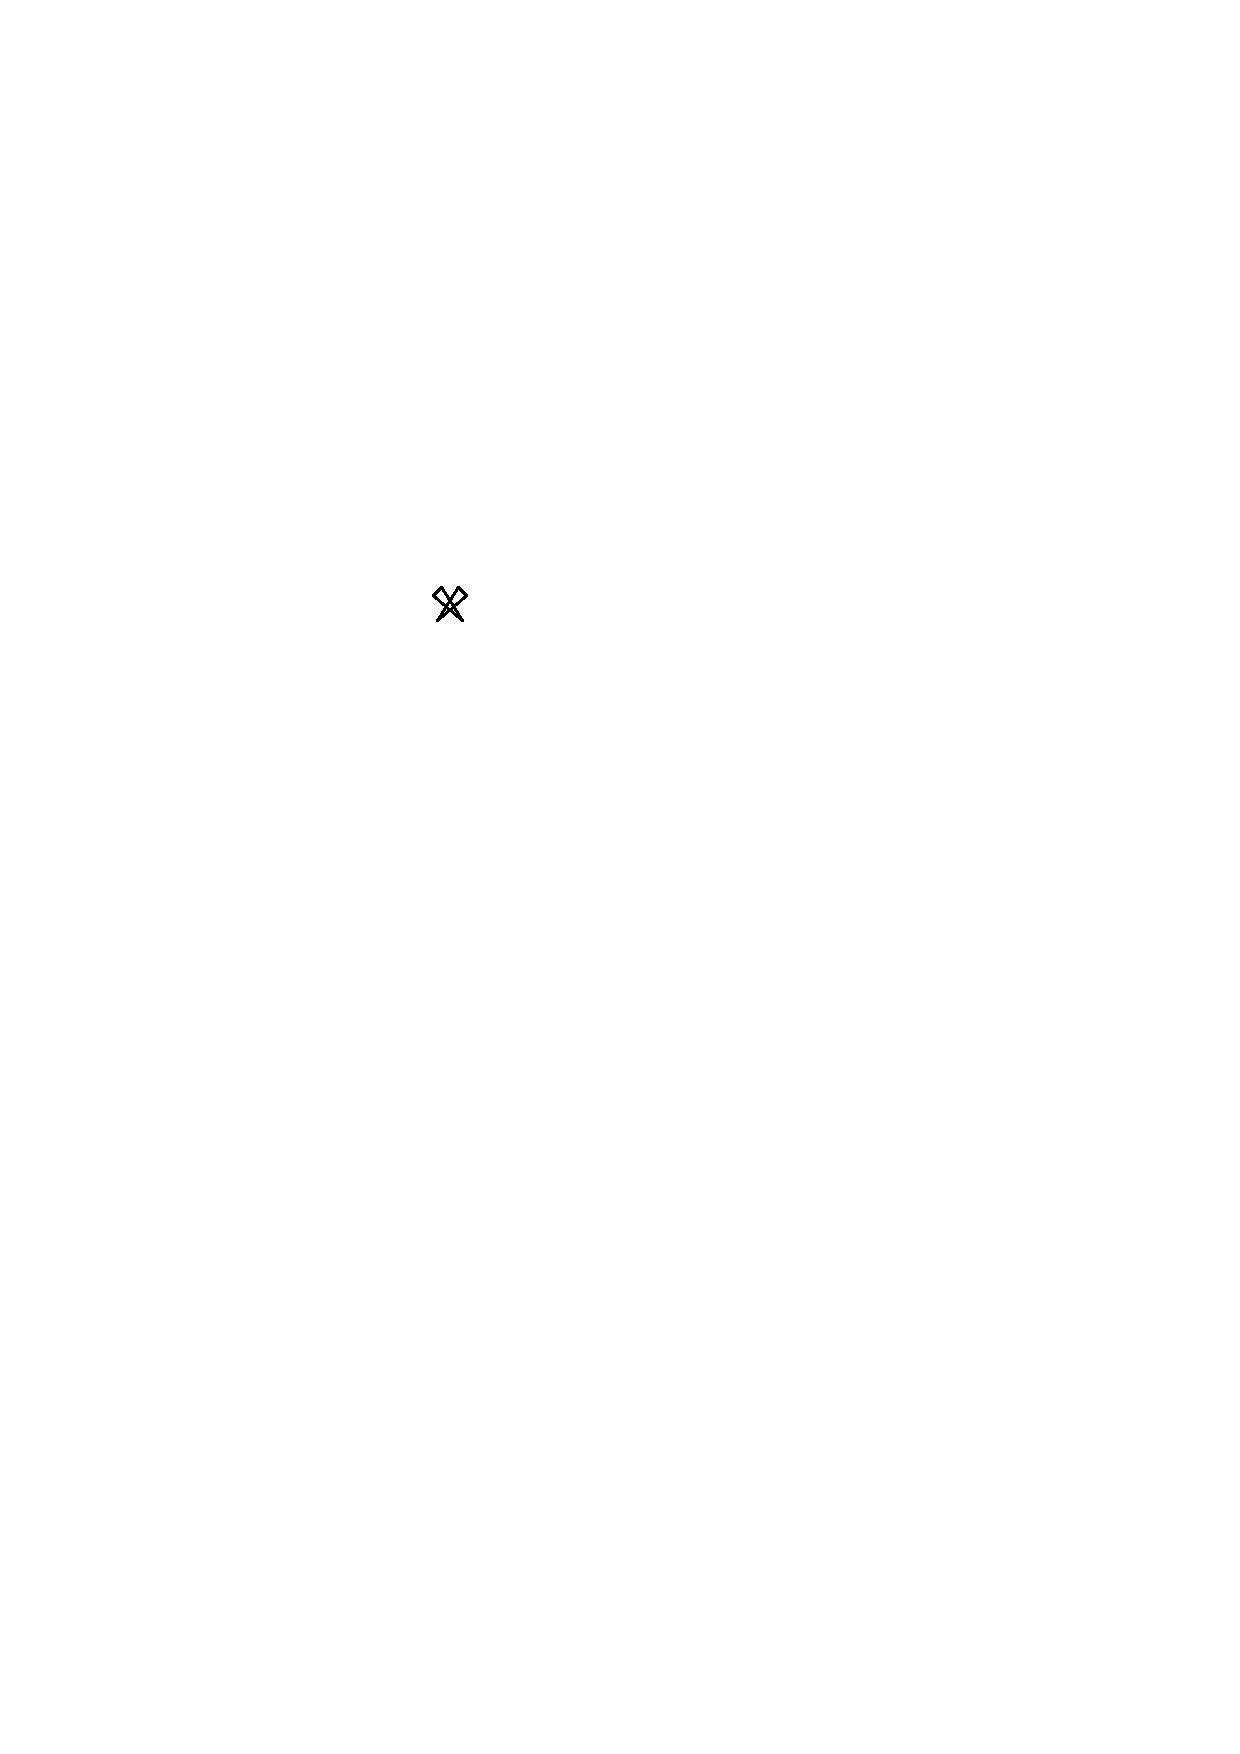
\includegraphics[height=1.6ex]{figs/triangles-disjoint-2}}}
\newcommand{\disjointc}{\raisebox{-.1ex}{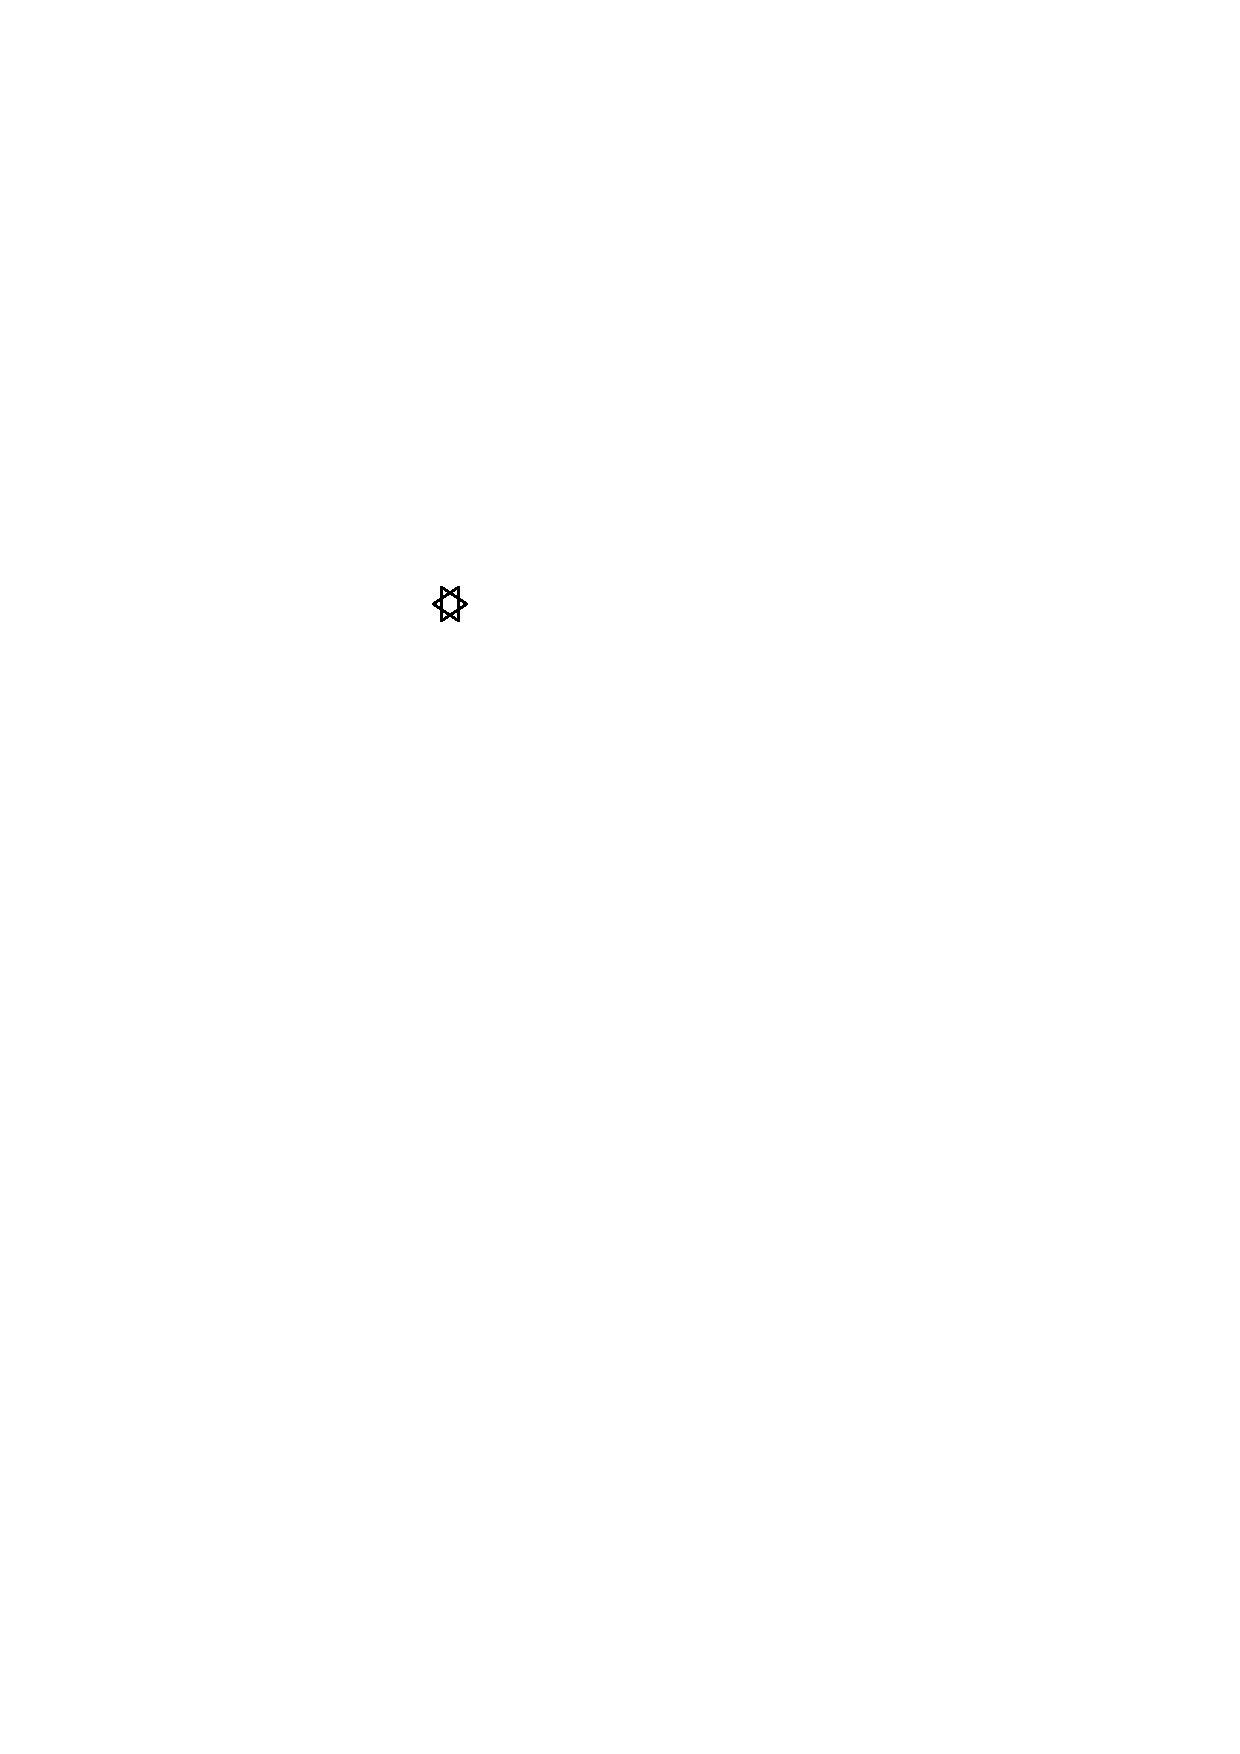
\includegraphics[height=1.6ex]{figs/triangles-disjoint-3}}}

\DeclareMathOperator{\ex}{ex}



%\usepackage{lineno}
%\linenumbers

\begin{document}
\maketitle

\begin{abstract}
  We study the following family of problems: Given a set of $n$ points
  in convex position, what is the maximum number triangles one can create
  having these points as vertices while avoiding certain \emph{forbidden
  configurations}.  As forbidden configurations we consider all 8 ways
  in which a pair of triangles in such a point set can interact.
\end{abstract}



\section{Introduction}

Let $t_1$ and $t_2$ be a pair of distinct triangles whose (4--6) vertices
are in convex position.  There are 8 combinatorially distinct ways that
these triangle can interact:  2 ways in which the triangles can share
an edge (\edgea\ and \edgeb), 3 ways in which the triangles can share a
single vertex (\vertexa, \vertexb, and \vertexc), and 3 ways in which
the triangles can have no vertices in common (\disjointa, \disjointb,
and \disjointc).

We consider the following class of problems:  Given a set, $X$,
of combinatorial configurations of pairs of triangles, what is the
largest set, $S$, of triangles one can create whose vertices are $n$
points in convex position, and such that no pair of triangles in $S$
forms a configuration in $X$.  We call the size of this set $\ex(n,X)$.
For example, 
\begin{equation}
    \ex(n,\{\edgea,\vertexb,\vertexc,\disjointb,\disjointc\}) = n-2 \enspace .
\end{equation}
This is because the set
$X=\{\edgea,\vertexb,\vertexc,\disjointb,\disjointc\}$ in this case
forbids any form of crossings between the edges of triangles. Thus,
the number maximum number of triangles we can have while avoiding $X$
is the number of triangles in a triangulation of a convex $n$-gon,
i.e., $n-2$. One of the results in this paper is that nearly the
same bound holds even if we allow the $\disjointb$ and $\disjointc$
configuration. In particular, our \thmref{blech} shows that
$\ex(n,\{\edgea,\vertexb,\vertexc\}) \in O(n\log n)$.



\begin{table}
\begin{center}
\begin{tabular}{ll}
  \hline
  $\ex(n,\{\edgeb\})\in \Theta(n^3)$ & \cite{brass:turan} \\
  $\ex(n,\{\edgea\})\in \Theta(n^2)$ & \cite{brass:turan} \\
  \hline
  $\ex(n,\{\vertexa\})\in \Theta(n^3)$ & \cite{brass:turan} \\
  $\ex(n,\{\vertexb\})\in \Theta(n^2)$ & \cite{brass:turan} \\
  $\ex(n,\{\vertexc\})\in \Theta(n^2)$ & \cite{brass:turan} \\
  \hline
  $\ex(n,\{\disjointa\})\in \Theta(n^3)$ & \cite{brass:turan} \\
  $\ex(n,\{\disjointb\})\in \Theta(n^2)$ & \cite{brass:turan} \\
  $\ex(n,\{\disjointc\})\in \Theta(n^2)$ & \cite{brass:turan} \\
  \hline
  $\ex(n,\{\vertexa,\vertexb\})\in \Theta(n^2)$ & \cite{brass:turan} \\
  $\ex(n,\{\vertexb,\vertexc\})\in \Theta(n^2)$ & \cite{brass:turan} \\
  $\ex(n,\{\vertexa,\vertexc\})\in \Theta(n^2)$ & \cite{brass:turan} \\
  \hline
  $\ex(n,\{\disjointa,\disjointb,\vertexa,\vertexb\}) = n$ & \cite{brass.rote.ea:triangles} \\
  \hline
  $\ex(n,\vertexa,\vertexb,\vertexc) \in \Theta(n)$ & from hypergraphs \\
  $\ex(n,\edgea,\edgeb) \in \Theta(n^2)$ & from hypergraphs \\
  $\ex(n,\disjointa,\disjointb,\disjointc) \in \Theta(n^2)$ & from hypergraphs \\ \hline
  $\ex(n,X\subset\{\edgea,\edgeb,\vertexa,\vertexb,\vertexc,\disjointa,\disjointb,\disjointc\}) \in \Omega(n)$ & here (contradicts \cite{brass.rote.ea:triangles}) \\
  $\ex(n,\{\edgea,\vertexb\}) \in \Omega(n^{3/2})$ & here \\
  $\ex(n,\{\edgea,\vertexb,\vertexa\}) \in \Omega(n^{3/2})$ & here \\
  $\ex(n,\{\edgea,\edgeb,\vertexb,\vertexa,\disjointa,\disjointb\}) \in \Omega(n^{3/2})$ & here \\
  $\ex(n,\{\edgea,\vertexb,\vertexc\}) \in \Omega(n) \cap O(n\log n)$ & \thmref{blech} \\
  $\ex(n,X\cup\{\edgeb\})\in \Theta(\ex(n,X))$ & \lemref{xcup} \\
  
  \end{tabular}
\end{center}
\caption{Known and new results on $\ex(n,X)$ for different sets $X$.}
\end{table}


\section{Some Easy Results}


\subsection{Edge-Sharing Non-Overlapping Triangles are Irrelevant}

The following lemma shows that including the $\edgea$ confguration in
the set $X$ of forbidden configurations has no effect on the asymptotics
of $\ex(n,X)$.

\begin{lem}\lemlabel{xcup}
   For any $X$, $\ex(n,X\cup\{\edgeb\}) \ge \ex(n,X)/8$.
\end{lem}

\begin{proof}
  Let $S$ be a set of triangles that achieves $\ex(n,X)$. For each pair
  of vertices $u$ and $w$ independently and uniformly choose a direction
  $\overrightarrow{uw}$ or $\overleftarrow{uw}$.  We then obtain a set
  $S'\subseteq S$ by removing any triangle that has a directed edge for
  which the triangle is to the left of the edge.  Observe that the set
  $S'$ does not contain a $\edgeb$ configuration.

  For any particular triangle $t\in S$, the probability that $t\in S'$
  is exactly $1/8$ since each of $t$'s three edges much be directed
  clockwise and edge directions are chosen independently.  By linearity of
  expectation, $\E[|S'|]=|S|/8=\ex(n,X)/8$.  We conclude therefore that
  there exists some subset $S''\subseteq S$ of size least $\ex(n,X)/8$
  that does not contain a $\edgeb$ configuration.  The set $S''$ proves
  that $\ex(n,X\cup\{\edgeb\}) \ge \ex(n,X)/8$.
\end{proof}

From this point onward, we will frequently include \edgeb\ in sets of
forbidden configurations when proving upper bounds.  By \lemref{xcup}
any upper bound we prove this way holds (within a factor of 8) without
including \edgeb.

\subsection{The Top/Bottom View}

It will be helpful to consider an top/bottom variant of $\ex(n,X)$
that is defined as follows (see \figref{top-bottom}).  Partition the
vertices of a convex $n$-gon using a horizontal line into a \emph{top
half} of size $\lfloor n/2\rfloor$ and a \emph{bottom half} of size
$\lceil n/2\rceil$.  We define $\ex'(n,X)$ analogously to $\ex(n,X)$
except that we only count triangles have one vertex in the bottom half
and one vertex in the top half.  When studying $\ex'$, each triangle
has a naturally defined \emph{bottom vertex} in the bottom half and a
\emph{left vertex} and \emph{right vertex}, each in the top half.

\begin{figure}
  \begin{center}
    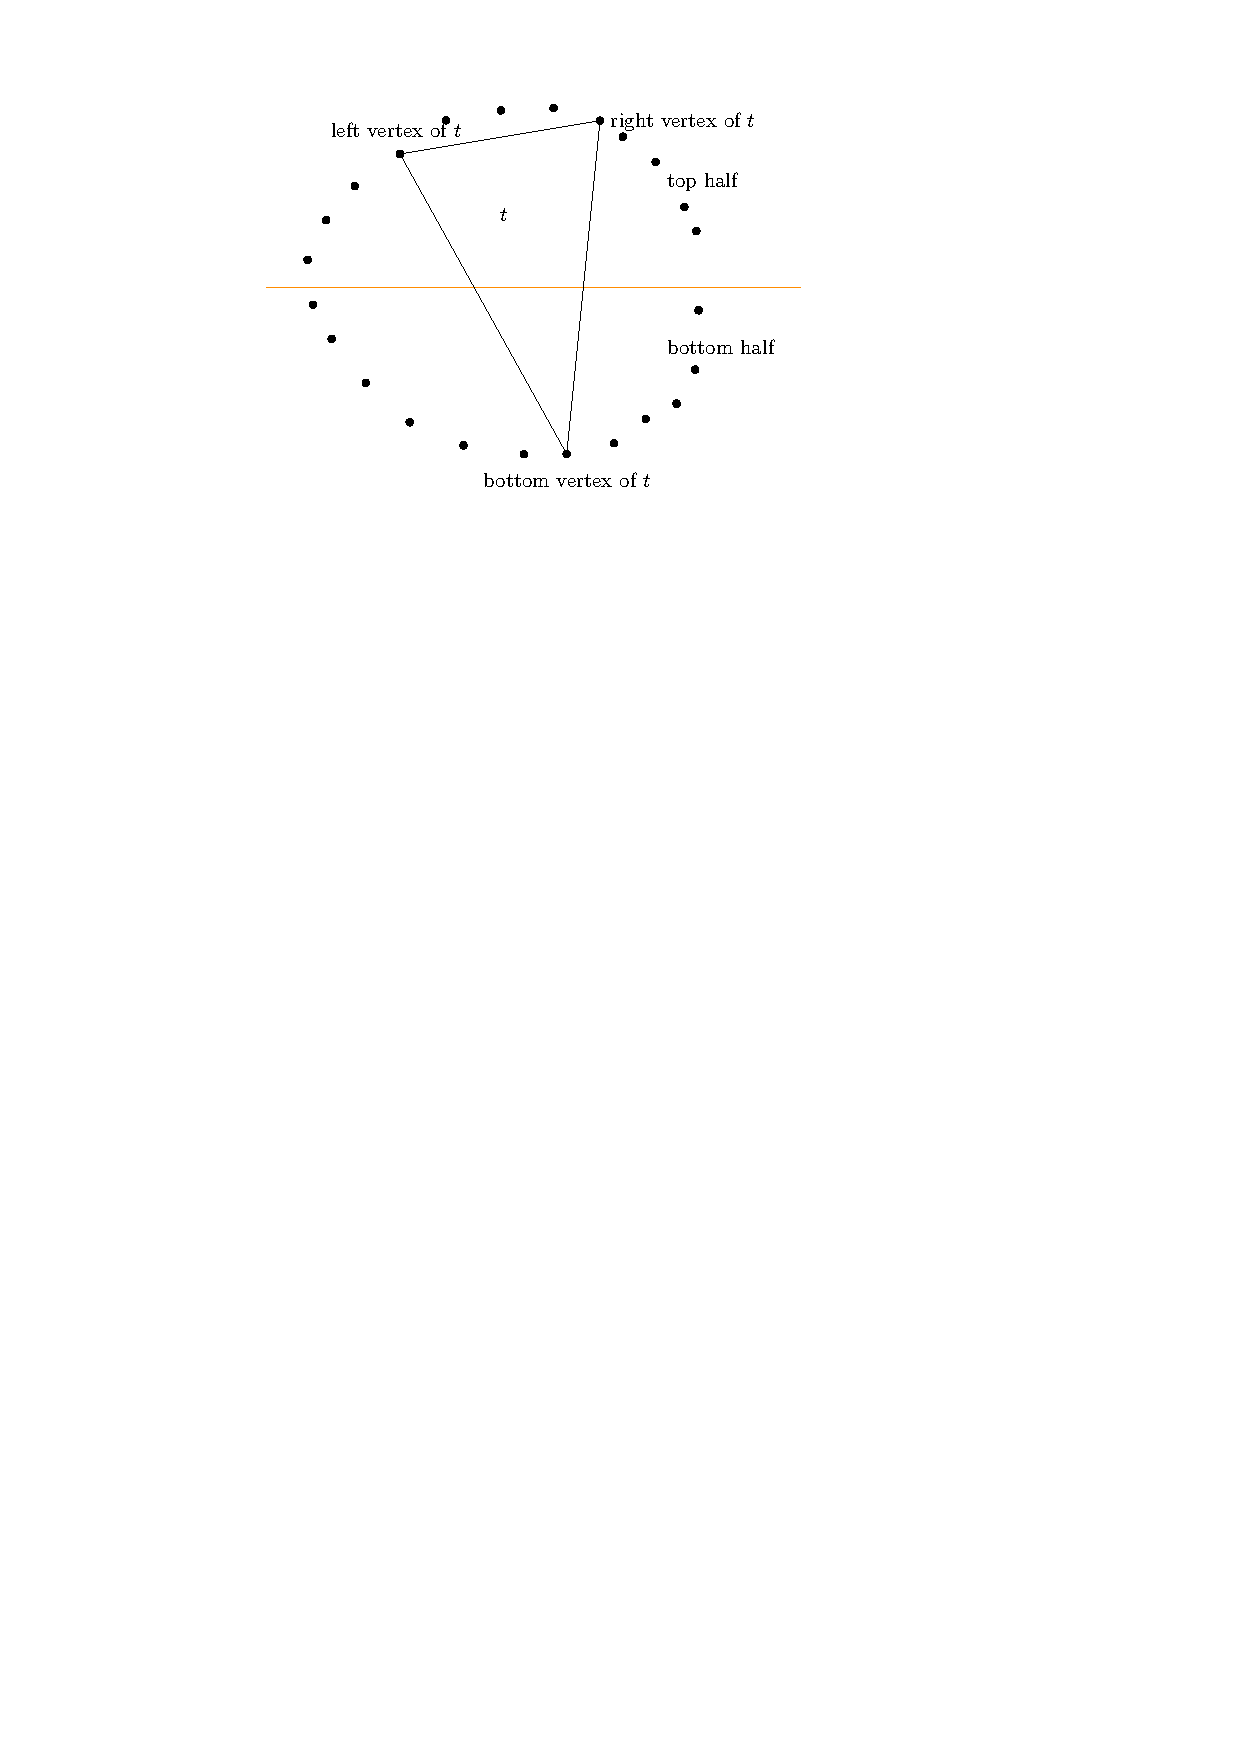
\includegraphics{figs/left-right}
  \end{center}
  \caption{$\ex'$ only counts triangles with two vertices in the top half
     and one vertex in the bottom half.}
  \figlabel{top-bottom}
\end{figure}

The following lemma shows that we can, without losing much, study $\ex'(n,X)$ instead of $\ex(n,X)$.

\begin{lem}\lemlabel{top-bottom}
  If $\ex'(n,X)\in O(n^c)$, then
\[
   \ex(n,X)\in 
      \begin{cases} 
          O(n^c)     & \text{if $c>1$} \\
          O(n\log n) & \text{if $c=1$}
      \end{cases}
\]
\end{lem}

\begin{proof}
   Let $S$ be a set of triangles that avoids $X$.  
   Every triangle in $S$
   is of one of the following types:
   \begin{enumerate}
      \item It has one vertex in the top half and two in the bottom half; there are $O(n^{c})$ such triangles.
      \item It has two vertices in the top half and one in the bottom half; there are $O(n^{c})$ such triangles.
      \item It has all three vertices in the top half; there are at most $\ex(\lfloor n/2\rfloor,X)$ such triangles.
      \item It has all three vertices in the bottom half; there are at most $\ex(\lceil n/2\rceil,X)$ such triangles.
   \end{enumerate}
   Thus, we obtain the recurrence inequality:
   \[  \ex(n,X) = O(n^{c}) + \ex(\lfloor n/2\rfloor,X) + \ex(\lceil n/2\rceil,X) \]
   which resolves to $O(n^c)$ for $c>1$ and $O(n\log n)$ for $c=1$.
\end{proof}


\subsection{The Dot Puzzle View}

It is sometimes helpful to take the top/bottom view of the problem
and turn it, instead, into a puzzle.  Refer to \figref{point-view}.
In this puzzle, we are given $\binom{n}{2}$ points,
\[
    Q = \{(x,y): y\in\{1,\ldots,n-1\}, x\in\{y+1,\ldots,n-1\} \} \enspace .
\]
These points model the top/bottom view on a set of size $2n$, where the
point $(x,y)$ represents a triangle whose vertices are some point on
the bottom and the $x$th and $y$th points on the top, where the top
vertices are labelled $1,\ldots,n$ from left to right.

\begin{figure}
   \begin{center}
      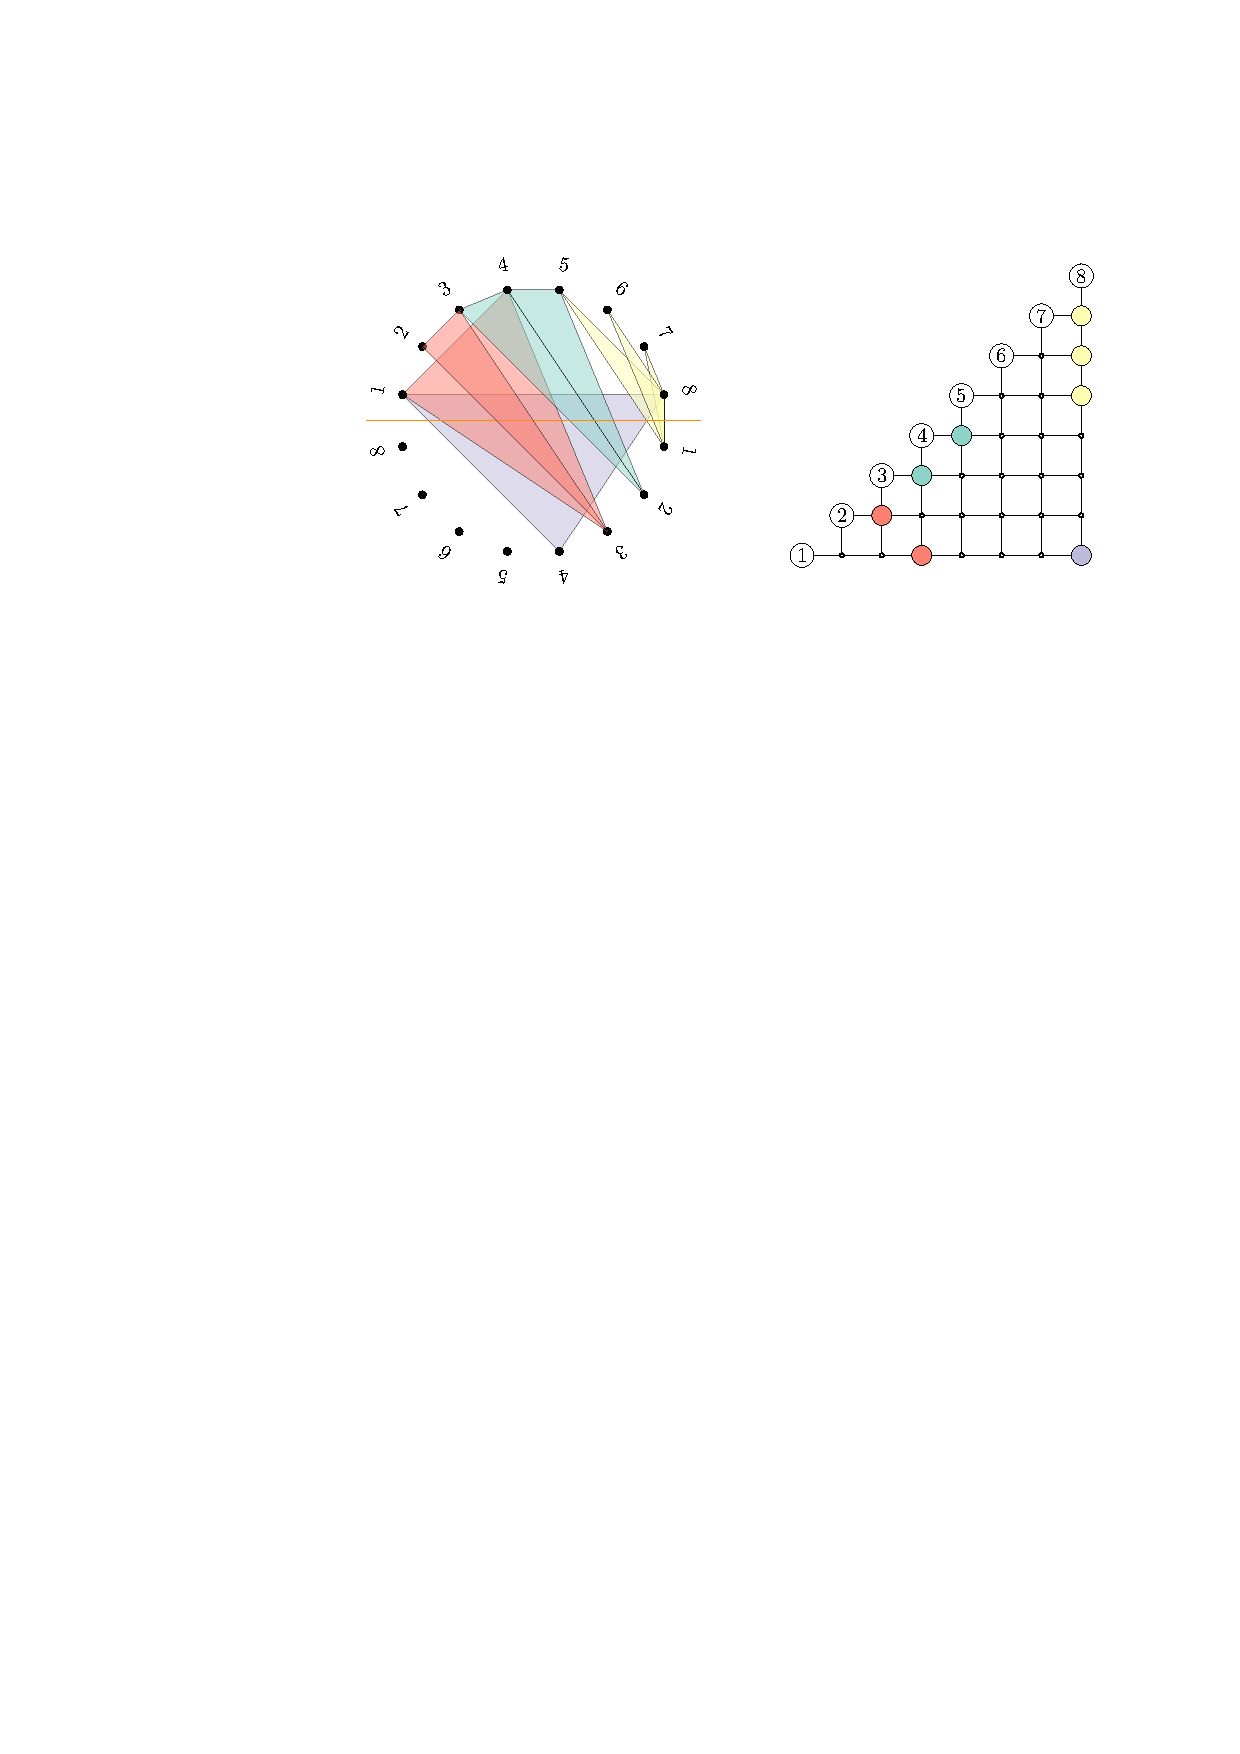
\includegraphics{figs/point-view}
   \end{center}
   \caption{The Dot Puzzle View of the Top/Bottom View. Orange points were
     selected in round 1, green points in round 2 and pink points in round 3.}
   \figlabel{point-view}
\end{figure}

The puzzle proceeds in $n$ rounds and during the $i$th round, the player
selects a set $Q_i\subseteq Q$ subject to certain constraints that depend
on the points selected in rounds $1,\ldots,i-1$.  In the top/bottom view,
the $i$th round determines which pairs of top vertices form a triangle
with the $i$th bottom vertex, where the bottom vertices are labelled
$1,\ldots,n$ from right to left.

Of course, the constraints imposed on the play of the game depend
on the set of forbidden configurations.  For example, the $\vertexb$
configuration adds two restrictions:
\begin{itemize}
   \item During a single round, we cannot select $(x_1,y_1)$ and
      $(x_2,y_2)$ with $y_1<y_2$ and $x_1>x_2$ since this would create
      a $\vertexb$ configuration at the bottom vertex.

   \item If $(x_1,y_1)$ is selected in some round, then we cannot,
      in a later round, select $(x_1,y_2)$ with $y_2<y_1$ nor can
      we select $(x_2,y_1)$ with $x_2<x_1$.  Doing so would create
      a $\vertexb$ configuration at the top vertex labelled $x_1$
      (respectively, at the top vertex labelled $y_1$).
\end{itemize}
For example, in \figref{point-view} the green triangle joining top
vertices 2 and 7 and the pink triangle joining top vertices 2 and 3
violate the second condition and these two triangles form $\vertexb$
configuration at top vertex 2.

The following table summarizes the constraints induced by various
configurations:

\begin{center}
\begin{tabular}{m{1em}|m{.45\textwidth}|m{.45\textwidth}}
      & killed by $(x,y)$ in subsequent rounds & killed by $(x,y)$
 in current round \\ \hline
$\edgea$ & $\{\}$
         & $x=y'$ \\ 
$\edgeb$ & $\{(x,y)\}$
         & $\{(x,y'):  y\neq y'\}$ \\
$\vertexa$ & $\{(x',y) : x'<x \}\cup\{(x,y') : y'<y \}$
         & $\{(x',y'): x < y'\}$ \\
$\vertexb$ & $\{(x',y) : x'<x \}\cup\{(x,y') : y'<y \}$
         & $\{(x',y'):x'<x, y'>y\}$ \\
$\vertexc$ & $\{(x',y) : x'>x \}\cup\{(x,y') : y'>y \}$
         & $\{(x',y'):y < y' < x < x'\}$ \\
$\disjointa$ & $\{(x',y'): x'< y\}$ 
         & $\{\}$ \\
$\disjointb$ & $\{(x',y'): y'> y\}$ 
         & $\{\}$ \\
$\disjointc$ & $\{(x',y'): y < y' <x,\,\, x'>x\}$
         & $\{\}$ \\
\end{tabular}
\end{center}
\section{Some Bounds}

Now, with our tools in hand, we are ready to study some problems.

\begin{thm}\thmlabel{blech}
  $\ex(n,\{\edgea,\vertexb,\vertexc\}) \in \Omega(n)\cap O(n\log n)$.
\end{thm}

\begin{proof}
  The $\Omega(n)$ lower bound is achievable by many constructions including,
  for example, any triangulation of a convex $n$-gon.

  To prove the $O(n\log n)$ upper bound, it suffices---by
  Lemmas~\ref{lem:xcup} and \ref{lem:top-bottom}---to show that
  $\ex'(n,\{\edgea,\vertexb,\vertexc,\edgeb\})\in O(n)$.

  We claim that each
  vertex in the top half is the left vertex of at most one triangle
  and is the right vertex of at most one triangle.  Therefore,
  each vertex of the top half is used in at most two triangles, so
  $\ex'(n,\{\edgea,\vertexb,\vertexc,\edgeb\}) \in O(n)$.

  Refer to \figref{triple-fig}.
  To see why each vertex in the top half is the left vertex of at most
  one triangle, observe that, since $\edgea$ and $\edgeb$ are forbidden
  configurations, the only other possibilties for two triangles to share
  a left vertex result in a $\vertexb$ or $\vertexc$ configuration.
  The argument for why each vertex is the right vertex of at most one
  triangle is symmetric.
  \begin{figure}
    \begin{center}
       \begin{tabular}{c@{\hspace{2em}}c}
          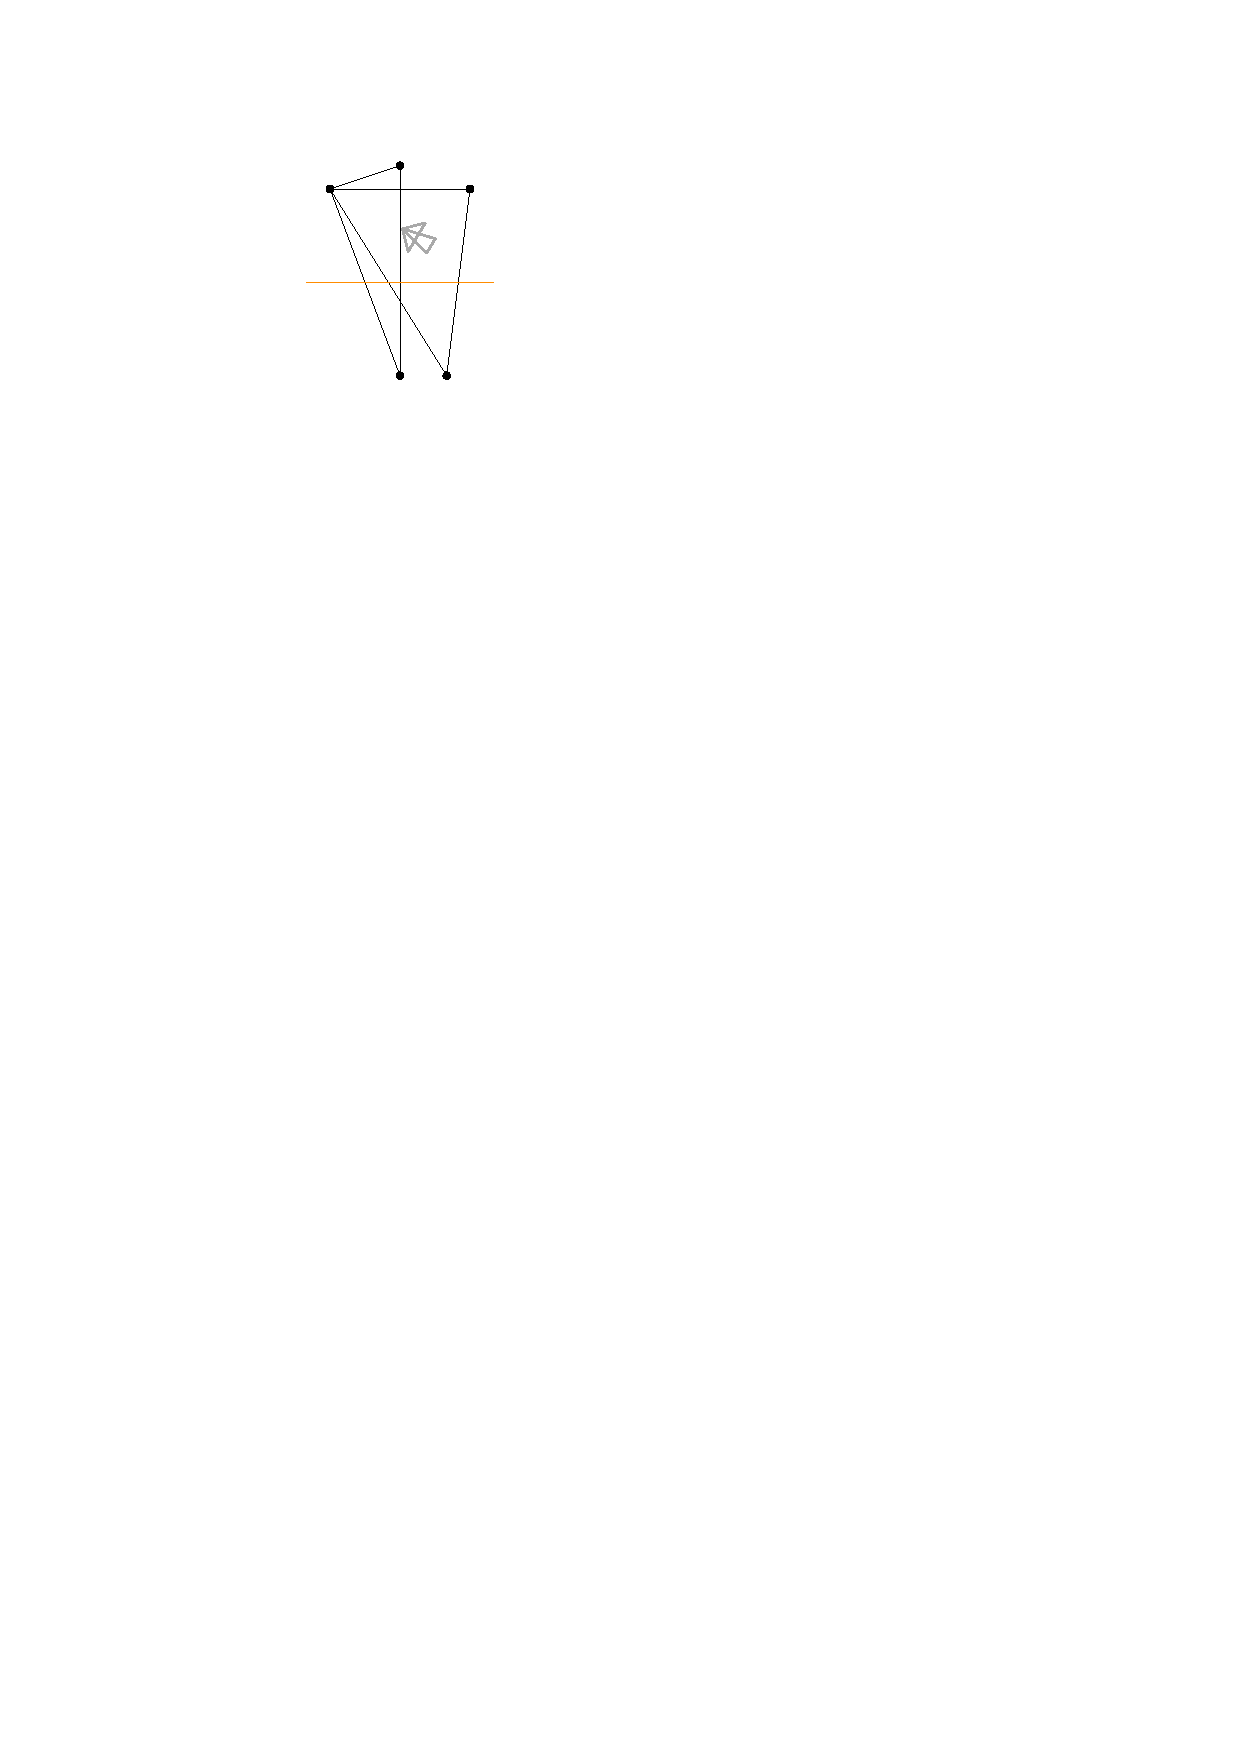
\includegraphics{figs/triple-fig-1} &
          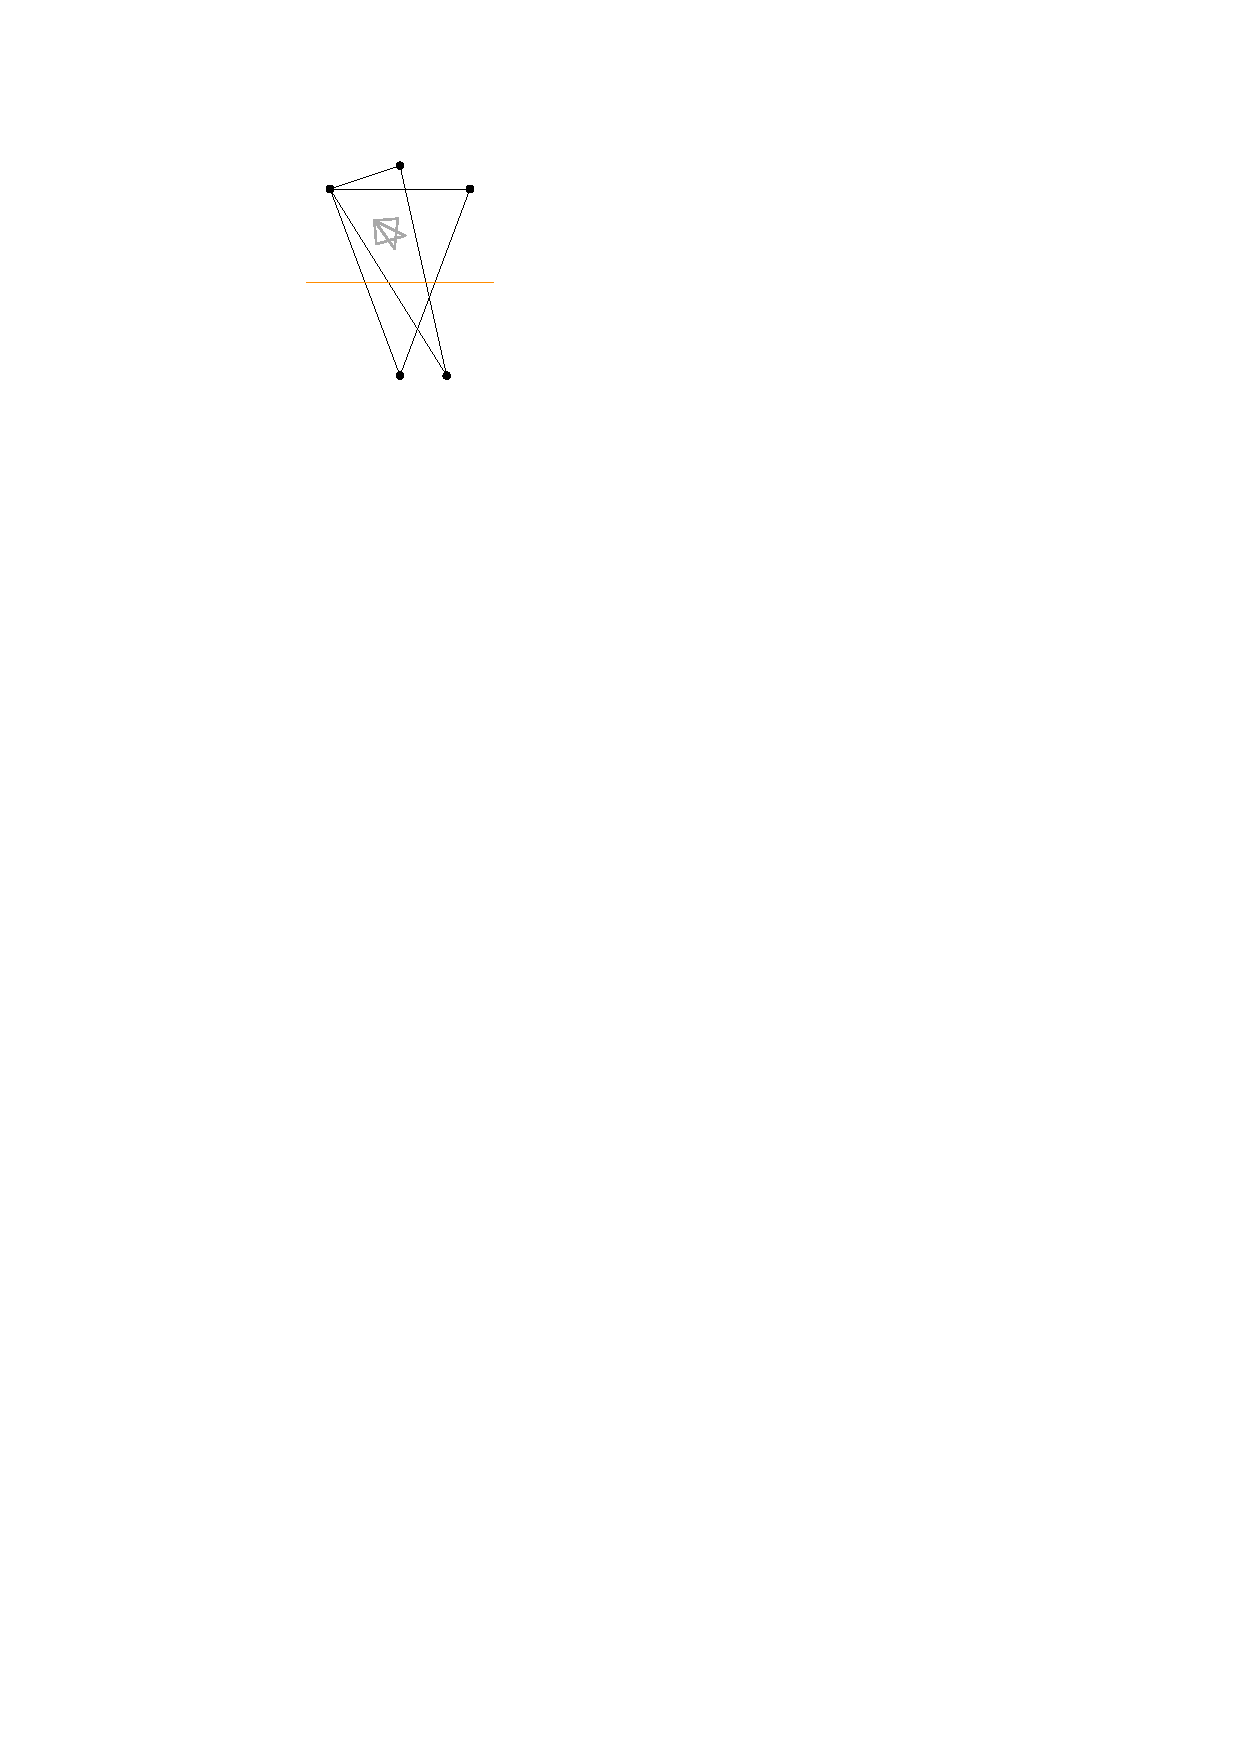
\includegraphics{figs/triple-fig-2} 
       \end{tabular}
    \end{center}
    \caption{Using a vertex as the left vertex of two triangles creates a 
      forbidden configuration}
  \end{figure}
  \figlabel{triple-fig}
\end{proof}

\bibliographystyle{plain}
\bibliography{turan}

\end{document}


